\documentclass[11pt]{article}
\usepackage{amsmath, amssymb, amsthm}
\usepackage{graphicx}
\usepackage{booktabs}
\usepackage[authoryear, round]{natbib}
\usepackage{hyperref}

\newtheorem{theorem}{Theorem}
\newtheorem{definition}{Definition}
\newtheorem{remark}{Remark}

\title{A short note on gradient descent}
\author{LaTeX Notes demo}
\date{}

\begin{document}

\maketitle

\begin{abstract}
Gradient descent is the simplest first-order method for minimising a differentiable function. This note states the method, proves its convergence rate for smooth convex functions, and illustrates how the step size affects progress. It is written as a demonstration document: every construct in it renders natively in Obsidian.
\end{abstract}

\section{The method}
\label{sec:method}

Let $f \colon \mathbb{R}^n \to \mathbb{R}$ be differentiable. Starting from a point $x_0$, gradient descent repeatedly moves against the gradient,
\begin{equation}
	x_{k+1} = x_k - \eta \, \nabla f(x_k),
	\label{eq:update}
\end{equation}
where $\eta > 0$ is the \emph{step size}. Each step is the minimiser of a simple quadratic model of $f$ around $x_k$, which is why the method is often described as following the direction of steepest descent \citep{boyd2004convex}.

\begin{definition}[$L$-smoothness]
\label{def:smooth}
A differentiable function $f$ is \textbf{$L$-smooth} if its gradient is $L$-Lipschitz:
\[
	\lVert \nabla f(x) - \nabla f(y) \rVert \le L \, \lVert x - y \rVert \quad \text{for all } x, y.
\]
\end{definition}

\section{Convergence}
\label{sec:convergence}

For smooth convex functions, gradient descent with a fixed step size converges at rate $O(1/k)$ \citep{nesterov2004introductory}.

\begin{theorem}[Sublinear rate]
\label{thm:rate}
Let $f$ be convex and $L$-smooth with minimiser $x^\star$, and run \eqref{eq:update} with $\eta = 1/L$. Then for every $k \ge 1$,
\begin{equation}
	f(x_k) - f(x^\star) \le \frac{L \, \lVert x_0 - x^\star \rVert^2}{2k}.
	\label{eq:rate}
\end{equation}
\end{theorem}

\begin{proof}
By smoothness, each step decreases the objective by at least a multiple of the squared gradient norm:
\begin{align}
	f(x_{k+1}) &\le f(x_k) - \frac{1}{2L} \lVert \nabla f(x_k) \rVert^2, \label{eq:descent} \\
	f(x_{k+1}) - f(x^\star) &\le \frac{L}{2} \left( \lVert x_k - x^\star \rVert^2 - \lVert x_{k+1} - x^\star \rVert^2 \right), \label{eq:telescope}
\end{align}
where the second line combines \eqref{eq:descent} with convexity. Summing \eqref{eq:telescope} over the first $k$ steps telescopes the right-hand side, and since the objective values are non-increasing, the bound in Theorem~\ref{thm:rate} follows.
\end{proof}

\begin{remark}
The step size matters. Section~\ref{sec:steps} shows what happens when it is too small or too large.
\end{remark}

\section{Choosing the step size}
\label{sec:steps}

Figure~\ref{fig:iterates} shows the iterates of \eqref{eq:update} on the one-dimensional quadratic $f(x) = x^2$, and Table~\ref{tab:steps} compares step sizes. A step size above $2/L$ makes the iterates diverge, which is why line search methods such as Armijo's rule are popular in practice \citep{armijo1966minimization}.

\begin{figure}[ht]
	\centering
	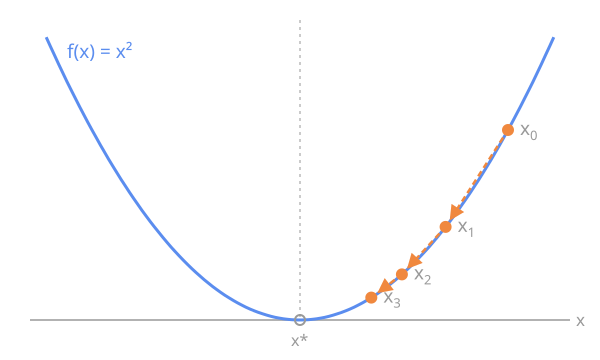
\includegraphics[width=0.75\linewidth]{iterates}
	\caption{Gradient descent on $f(x) = x^2$ with $\eta = 0.15$: each step shrinks the distance to the minimiser by the same factor, $1 - 2\eta = 0.7$.}
	\label{fig:iterates}
\end{figure}

\begin{table}[ht]
	\centering
	\begin{tabular}{lll}
		\toprule
		Step size $\eta$ & Behaviour on $f(x) = x^2$ & Iterations to $|x_k| < 10^{-6}$ \\
		\midrule
		$0.05$ & slow, monotone & $132$ \\
		$0.30$ & fast, monotone & $16$ \\
		$0.50$ & exact in one step & $1$ \\
		$0.90$ & oscillating, converging & $62$ \\
		$1.10$ & diverging & --- \\
		\bottomrule
	\end{tabular}
	\caption{Effect of the step size, starting from $x_0 = 1$ (here $L = 2$).}
	\label{tab:steps}
\end{table}

\section{Summary}

\begin{itemize}
	\item The update \eqref{eq:update} needs only gradients.
	\item With $\eta = 1/L$ it achieves the rate \eqref{eq:rate} on smooth convex functions (Theorem~\ref{thm:rate}).
	\item Too large a step size breaks convergence (Section~\ref{sec:steps}).
\end{itemize}

\bibliographystyle{abbrvnat}
\bibliography{references}

\end{document}
